\documentclass[journal]{IEEEtran}
\usepackage[a5paper, margin=10mm, onecolumn]{geometry}
\usepackage[cmex10]{amsmath}
\usepackage{amssymb,amsfonts,amsthm}
\usepackage{gvv-book}
\usepackage{gvv}
\usepackage{hyperref}
\usepackage{physics}
\usepackage{gauss}

\begin{document}
\title{4.2.28}
\author{EE25BTECH11025 - Ganachari Vishwambhar}
\maketitle

\textbf{Question}:\\
Solve the system of linear equations:
\begin{align}
    5x-8y=-1\\
    3x-\frac{24}{5}y=\frac{-3}{5}
\end{align}
\textbf{Solution: }\\
Given:
\begin{align}
    \myvec{5&-8}\vec{x}=-1;\myvec{3&\brak{\frac{-24}{5}}}\vec{x}=\frac{-3}{5}\\
    A=\myvec{5&-8\\3&\brak{\frac{-24}{5}}};
    \vec{x}=\myvec{x\\y};
    \vec{b}=\myvec{-1\\ \brak{\frac{-3}{5}}}\\
    A\vec{x}=\vec{b}
\end{align}
Let:\\
Rank of coefficient matrix $=r$\\
Rank of Augmented matrix $=r_a$\\
Order of coefficient matrix $=n$\\
Augmented Matrix:
\begin{align}
    \augvec{2}{1}{5&-8&-1\\3&\brak{\frac{-24}{5}}&\brak{\frac{-3}{5}}}\\R_2 \rightarrow R_2-\frac{3}{5}R_1\\
    \augvec{2}{1}{5&-8&-1\\0&0&0}\\
    r=1;r_a=1;n=2\\
    \because r=r_a<n
\end{align}
Infinite solutions exist for the given system of linear equations.

\begin{figure}[h!]
   \centering
   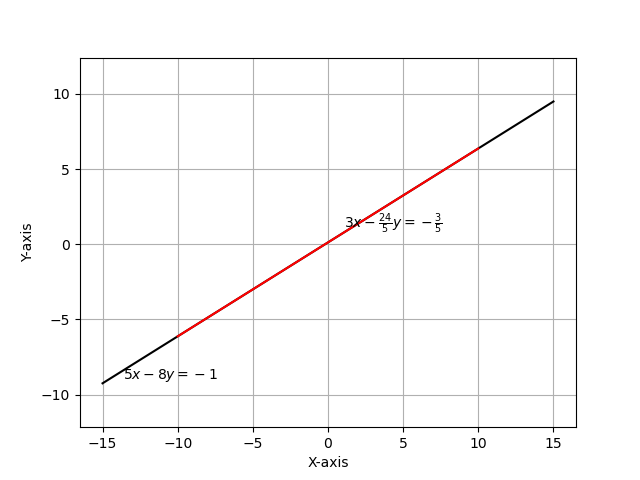
\includegraphics[width=0.7\linewidth]{figs/plot.png}
   \caption{Plot of the given system of lines}
   \label{}
\end{figure}
\end{document}  